\section{Softwarearkitektur}
Dette afsnit beskriver softwarearkitekturen. For at give det fornødne overblik over softwarearkitekturen i vores system, har vi valgt at inkludere en overordnet domænemodel, en domænemodel for software samt et tomt klassediagram uden attributter og metoder. I afsnittet design findes sekvensdiagram og klassediagram for UC1. Diagrammer er med til at danne grundlaget for software designprocessen. Ved at man bryder systemet ned i mindre dele, giver det tilmed også et overblik over hvad der skal foregå i systemet, og dette gør det nemmere at finde frem til designløsninger. Nedenstående figur den overordnede domænemodel, som giver et overblik og hele systemet. 

\subsection{Overordnet domænemodel}
	\begin{figure}[h!]
	\centering
	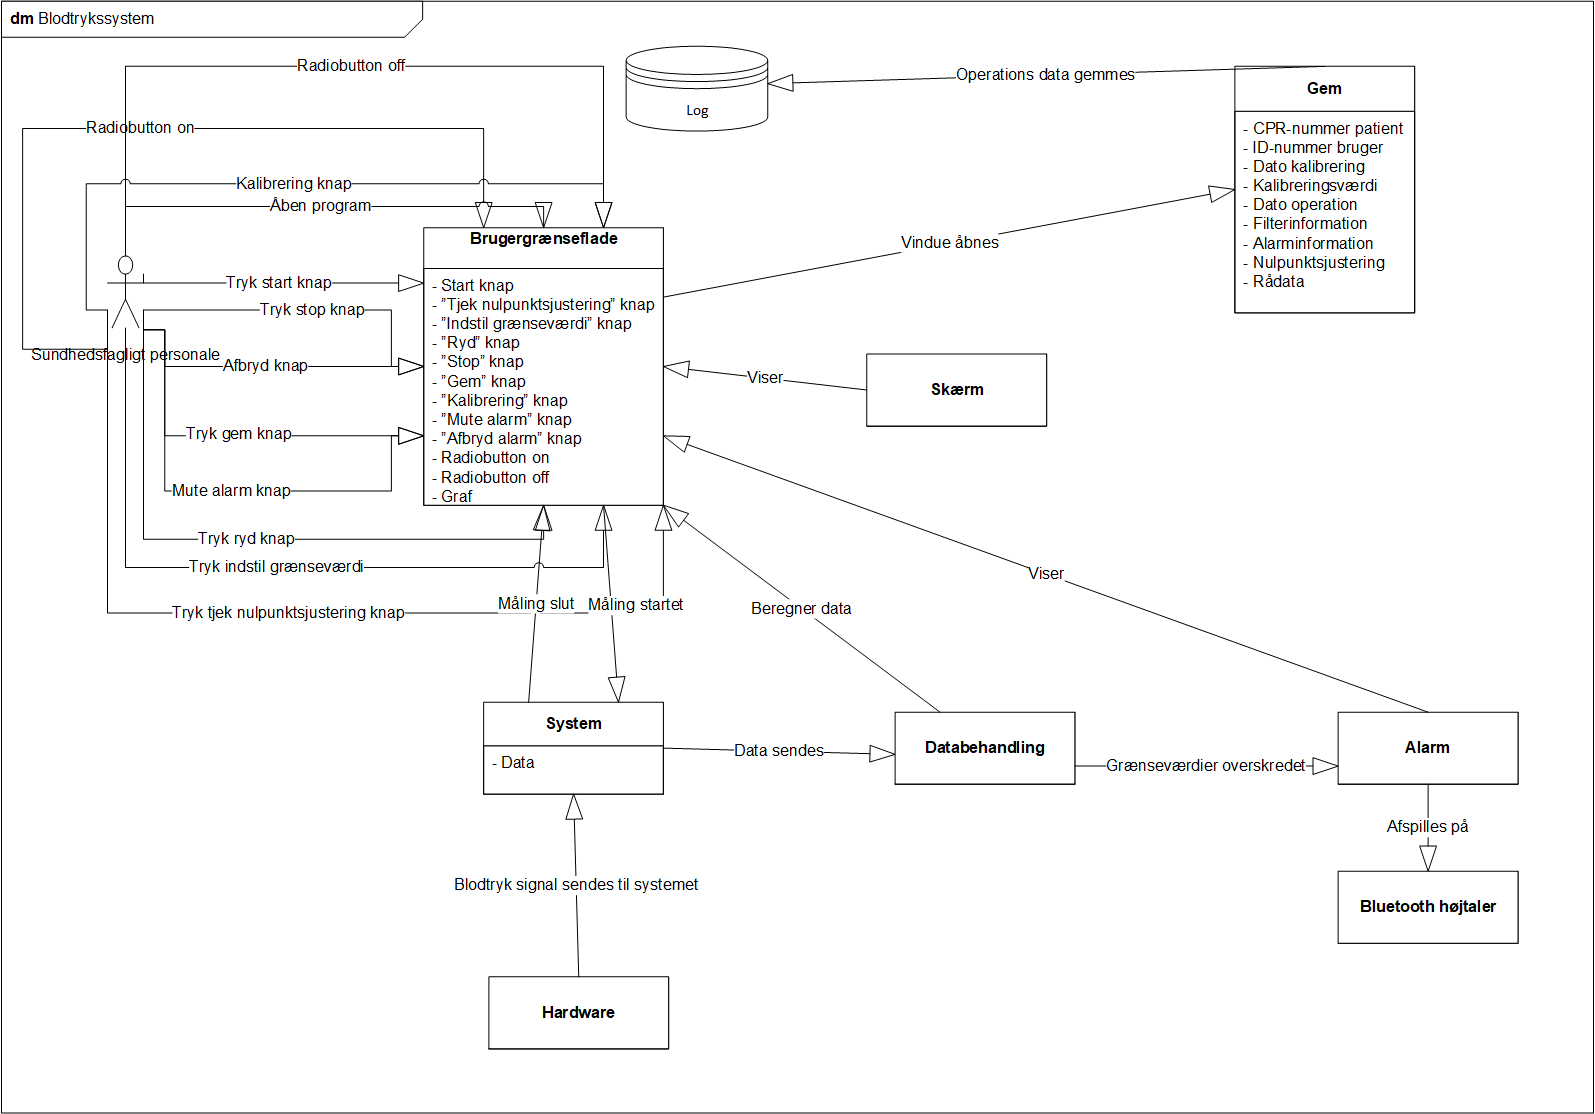
\includegraphics[width=1\linewidth]{Arkitektur_og_design/Softwarearkitektur/overordnetdomain}
	\label{fig:overordnetdomain}
	\caption{Overordnet domænemodel}
\end{figure}

Ovenstående figur \vref{fig:overordnetdomain} illustrerer den overordnede domænemodel, som viser både hardware og software. Domæneklassrne fandt vi efter en navneords analyse af vores fully dressed use cases, hvor vi fandt frem til brugergrænseflade, sundhedsfagligt personale, log, skærm, gem, system, databehandling, alarm og bluetooth højtaler.  Log domænet er en tekstfil, hvor oplysninger fra operationen gemmes i.

\subsection{Domænemodel for software}
  
Ud fra vores kendskab til domænet, har vi lavet en software-domænemodel, hvor vi får et overblik over, hvilke domæneklasser vores software skal indeholde. 

\clearpage

\begin{figure}[h!]
	\centering
	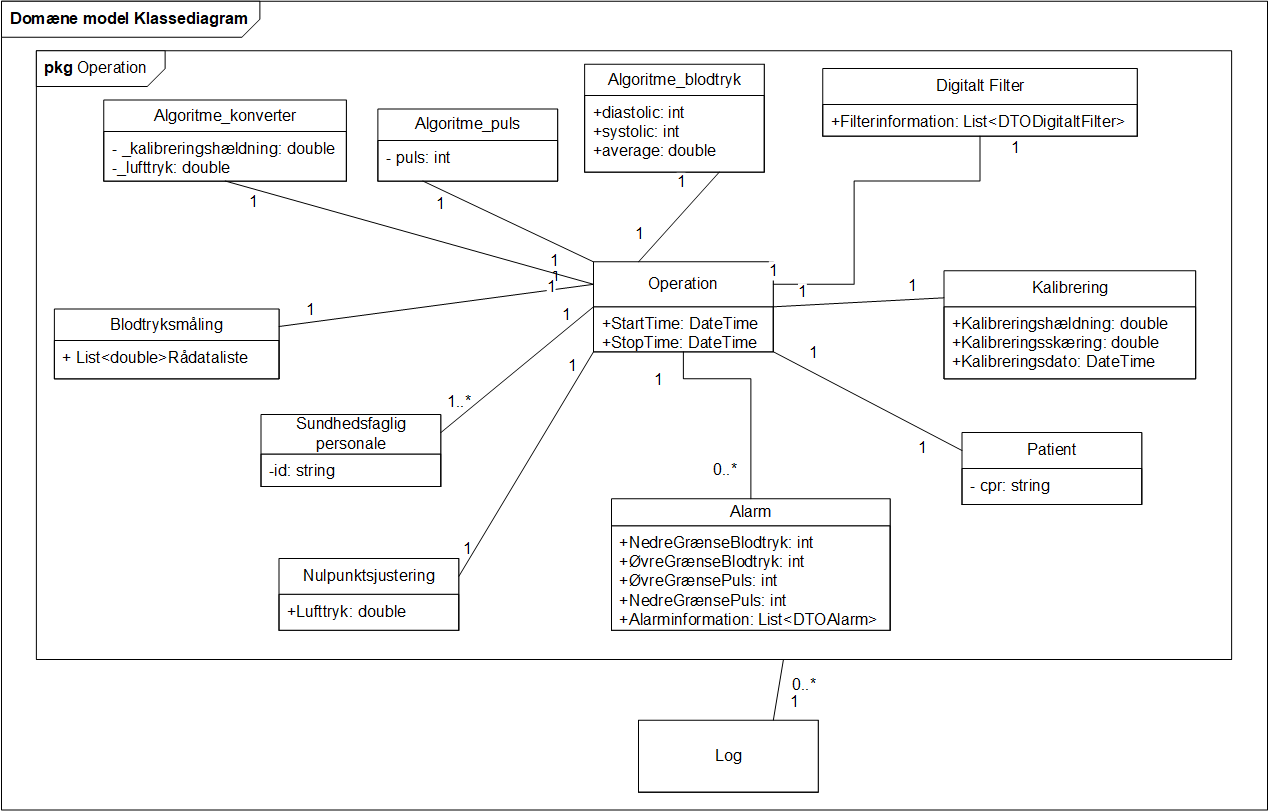
\includegraphics[width=1\linewidth]{Arkitektur_og_design/Softwarearkitektur/classdomain}
	\label{fig:classdomain}
	\caption{Domænemodel for software}
\end{figure}

Ovenstående figur \vref{fig:classdomain} viser systemets domæne for softwaren og hvilke klasser dette er bestående af.  Herudover viser den relationen mellem de forskellige domæneklasser og operationen. For eksempel kan der ved 1 operation være 0 til mange alarmer, som er illustreret ved "0..*". Modellen viser også en oversigt over klassernes tilhørende attributter og typerne af disse. Typerne har vi rationaliseret os frem til ved viden om at vores målinger vil være decimaltal (doubles), vores beregner vil vi gerne have vist i heltal (int), id og cpr er hensigtmæssigt at gemme som en string, og så vi nogle start- og stoptidspunkter som er oplagte at lave som DateTime. 

Ud fra vores use cases er vi kommet frem til, at ovenstående domæneklasser kan beskrive vores domæne tilstrækkeligt. Det gjorde vi, som tidligere nævnt, ved at lave en navnordsanalyse af vores fullydressed use cases. Ud fra denne fandt vi domæneklasserne: sundhedsfagligt personale, nulpunktsjustering, patient, alarm, kalibrering, digitalt filter, blodtryksmåling samt log. Ud fra disse gav det mening at samle det hele under klassen operation, som er vores brugssituation. Vi indså, at vi manglede klasser for vores databehandling. Dette delte vi op i tre klasser. En til pulsalgoritme, en til blodstryksalgoritme og en klasse til at konvertere fra volt til mmHg. 

Dernæst lavede vi et overordnet tomt klassediagram, som er udformet på baggrund af vores use cases. Klasserne fra software domænemodellen er en del af vores Model package, som indeholder domæneklasser og dtoklasser. 

\clearpage

\begin{figure}[h!]
	\centering
	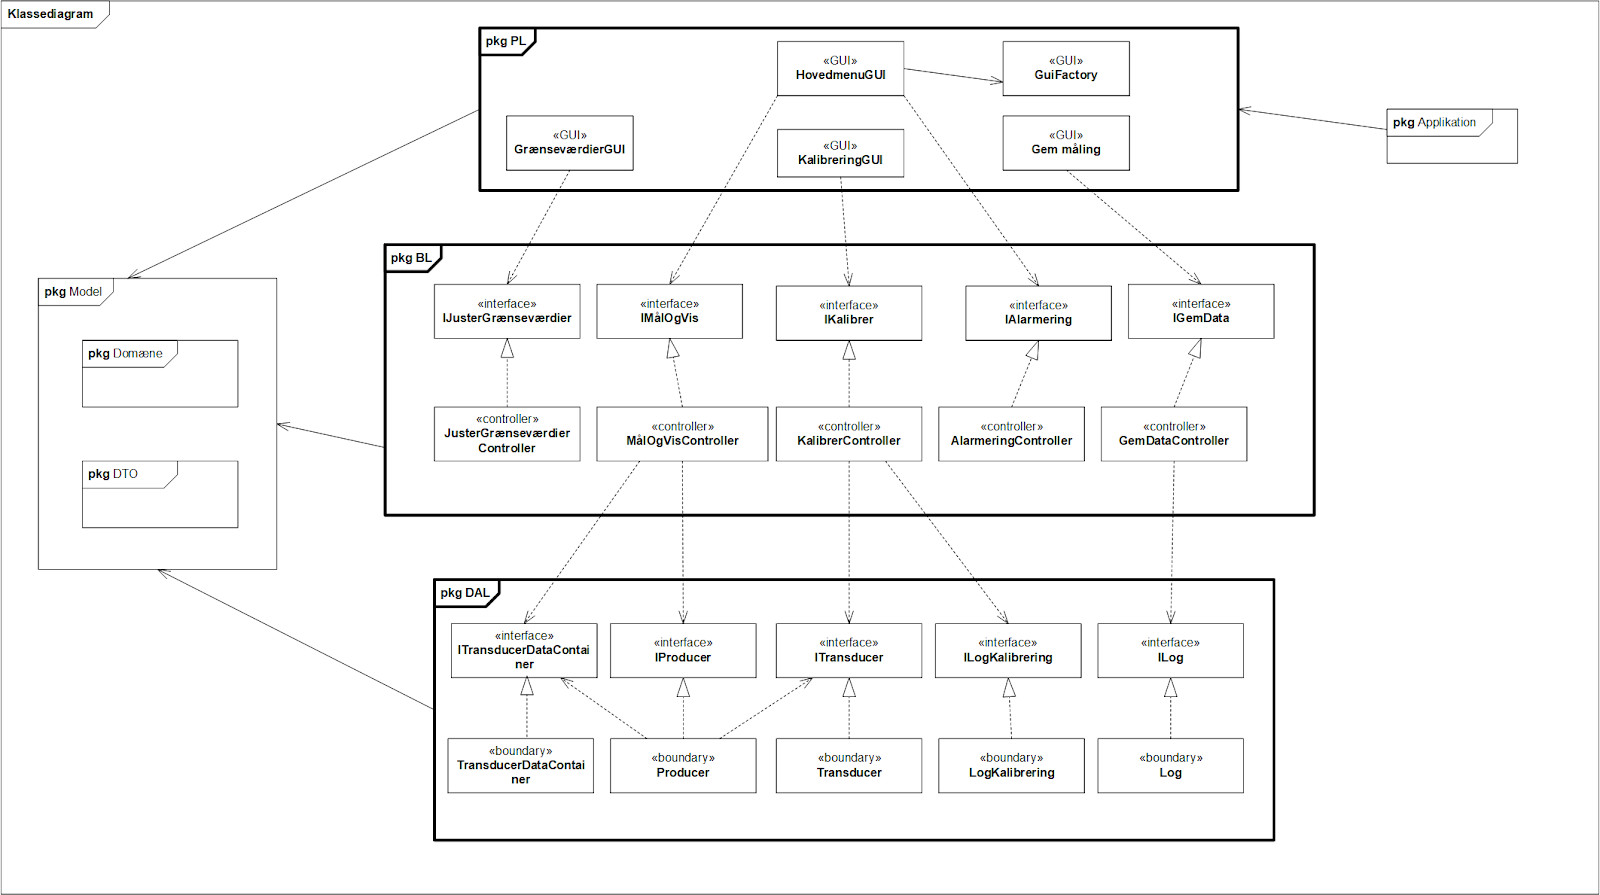
\includegraphics[width=1\linewidth]{Arkitektur_og_design/Softwarearkitektur/tomclass}
	\label{fig:tomclass}
	\caption{Klassediagram uden attributter og metoder}
\end{figure}

Klassediagrammet på figur \vref{fig:tomclass} viser opbygningen af softwaren. Vi har valgt at bygge vores system op efter trelagsmodellen, med præsentationslag (PL), businesslag (BL) og datalag (DAL). Dette er en god opbygning af et større system, som skal indhente, behandle og vise data.

Klassediagrammet viser opbygningen af softwaren. Vi har valgt at bygge vores system op efter trelagsmodellen, med præsentationslag (PL), businesslag (BL) og datalag (DAL). Dette er en god opbygning af et større system, som skal indhente, behandle og vise data. 

Klasserne fra software domænemodellen er en del af vores Domæne package, som ligger i vores Model package, der også indeholder en DTO package, som består af fem dtoklasser. En for alarm der skal bruges til at gemme alarmtype og tidspunkt for en alarm, en for blodtryksberegninger som bruges til at sende beregninger fra BL til PL, en for digitalt filter der skal bruges i forbindelse med logging af filterstatus i løbet af en måling, en DTO med alle properties der skal gemme i loggen og en for kalibrering. Sidst men ikke mindst er der en package kaldet Applikation, som står for at starte hele applikationen op. 

Softwaren er designet ud fra paradigmet om lav kobling. Dette er først og fremmest gjort ved, at dele de forskellige use cases op i egne klasser med interfaces imellem for at opfylde open-closed princippet. Derudover er der brugt dependency injection, som ligeledes fremmer en lav kobling. Denne opbygning gør det også muligt at benytte scrum  da hver use case har sin egen klasse i softwaren, og man dermed kan arbejde individuelt på hver sin use case. Desuden bliver det også lettere at teste og lokalisere eventuelle fejl. Derudover er det i fremtiden, lettere at genbruge softwaren i nye applikationer, samt at udvide uden at skulle lave alt for mange ændringer i koden. 

Et knudepunkt i softwaren er klassen HovedmenuGUI, som har mange ansvar. Dette ansvar er forsøgt mindsket ved at lave en GuiFactory klasse, som sørger for at oprette instanser af de tre andre GUI’er. Dette sikrer også, at det ville være nemt at tilføje en anden GUI, hvis softwaren skal udvides med en ny funktionalitet. 

Kommunikationen mellem datalaget og logiklaget er designet ud fra producer-consumer princippet. Dette var en oplagt løsning, da vores måleenhed hele tiden producerer data, som skal bruges og behandles af controllerklasserne i logiklaget. En anden vigtig feature ved producer-consumer er, at en datakø er indbygget, som sørger for, at der ikke går måledata tabt mellem datalaget og logiklaget, som kører i hver sin tråd. Køen har vi realiseret ved at bruge AutoResetEvents, som forhindrer, at producertråden overskriver måledata, inden de er blevet consumed i logiklaget. På den måde undgås fejl i kommunikationen mellem datalaget og logiklaget.

Mellem logiklaget og præsentationslaget var det i første omgang planen at bruge observer pattern. Det viste sig dog, at dette ikke var særlig hensigtsmæssigt, da der er forskel på, hvor tit blodtryksgrafen og beregningerne på hovedmenuen skal opdateres. Dette gjorde det vanskeligt at bruge observer standardmønstret. Der var behov for en mere generisk løsning. Kommunikationen mellem logiklaget og præsentationslaget blev i stedet løst ved at bruge events, som på mange måder minder om observer, men er en mere fleksibel metode, der er indbygget i .NET frameworket. Dette viste sig også at være en god løsning på kommunikation mellem alarmeringscontrolleren og hovedmenuen. Her blev der altså afgivet fra ASE-modellen, da der blev arbejdet iterativt med software arkitekturen. Det fleste ændringer har dog været mindre ændringer som fx tilføjelse af flere klasser i datalaget. Se dokumentet softwarearkitektur og design hvor den første version af klassediagrammet kan findes.  

En anden udfordring var en samplefrekvens på 1000 Hz og en computerskærm, der opdaterer med 60 Hz. For at undgå en nedsampling af signalet i softwaren, blev det besluttet, at grafen opdaterer med 100 punkter af gangen 10 gange i sekundet. Opdateringsfrekvensen på skærmen bliver således kun 10 Hz. Blodtryksgrafen opdaterer altså ikke helt så smooth, men dette blev besluttet som et fint kompromis, da der ikke mistes information i signalet på grund nedsampling. 
